\chapter{Requirements Analysis}\label{C:ra}
To guide the creation of the visualisation a user oriented design approach was used, in particular making use of user models (personas) which were created to give a sense of empathy and understanding for the foreseen users of the visualisation in order to better understand the requirements and design decisions to be made. 

The design of the visualisation was based heavily on User Centered Design as it provided a method of user interface design as well as visualisation design. User Centered Design is a process in which the needs, wants, and limitations of the end users of a system are given extensive attention. To achieve this, personas were created (also known as archetypal users), which are a personification the needs of a larger group of related users. These personas act as stand-ins for real users, describing them in terms of their goals and personal characteristics, and although they are fictitious, they are based on knowledge of real users. This design methodology supported my understanding of how users were likely to use the visualisation.
\\\\
An additional tool used during requirements analysis was User Scenarios which describe the foreseeable interactions of the user personas with the visualisation. A scenario is made up of a functional goal for the visualisation and describes how it is carried out by a persona. Both of these tools force you to think about the tasks needed for the visualisation and their context in the system as a whole. Once the personas and scenarios have been completed you can then start to design specific elements of the user interface and visualisation based on the requirements and interactions described in the scenarios.
\section{User models}
Below are the two personas that were used in the design of the visualisation for this project. They depict users that would use the visualisation in the context of a terminal or display in an observatory environment. These personas  can be validated during evaluation of the visualization by finding real users that match the core values of the personas.

\subsection{John Truman (Primary Persona - The interested layperson)}\
24 year old John is interested in planets and space and has a basic knowledge about both. He frequently visits attractions catering to this interest at locations such as planetariums and observatories. Some of his favourite things to do when visiting these attractions is to go to the computer terminals that allow users to choose what information they see.

John is used to playing computer games and using visualisations and is not overwhelmed understanding and using new systems. He finds that he learns better when provided with visual examples than when reading or listening to information. John is most comfortable using keyboard and mouse when interacting with a computer.
\subsection{Cara Thompson (Secondary Persona - Likes gesture based systems)}
23 year old Cara likes using interactive visualisations when visiting attractions, she finds that they are more entertaining and provide a better level of interaction and more of a novelty experience with a visualisation than simply a keyboard and mouse. 
\\\\
Both of these users are similar in their need for information from the visualisation but differ in the methods that they wish to access the information and interact with the visualisation. John wants to interact with keyboard and mouse as it is more straight forward and accurate. Cara wants to interact with gestures as she finds it more of a novelty and more immersive.
\section{Scenarios}
 A good use scenario does a number of things:
\begin{itemize}
 \item Describes the user's goals and motivations.
  \item Describes a specific task or tasks that need to be accomplished.
   \item Describes some of the interaction, with enough detail to make it compelling, but not so much detail as to be overwhelming.
    \item Provides a shared understanding for everyone on your team about what a user might want to do and how they might do it.
     \item Helps you construct the sequence of events that are necessary to address in your user interface.
     \item Can be sketchy, as long as it provokes ideas and discussion.
\end{itemize}
 \subsection{Scenario 1: View planets ordered by their similarity to Earth}
   {\bf Primary Persona:}\\
 When John first sees the system the first thing he notices is that their are many planets orbiting what looks like a star. He doesn't have any point of reference for these planets so their sizes, colours, and movement speeds are meaningless. By providing a way of comparing the planets to Earth it gives a point of reference which is well documented and known by most.
 
 {\bf Procedure:}
 \begin{enumerate}
 \item John clicks a prominent button stating view planet similarity to earth.
 \item The planets on screen move so that the earth is located at the center and top of the screen with all others orbiting it. The planets with a high internal similarity to earth are higher on the Y axis whilst the planets with a high surface similarity to earth are closer to the center of the orbiting planets on the X axis.
 \item From here John can select any of the planets for further analysis.
 \end{enumerate}
 \subsection{Scenario 2: Select ranges for attributes of each planet displayed}
   {\bf Primary Persona:}\\
 John has become comfortable with selecting the planets and has some idea of the scale and basic attributes of the planets. Now he wants to select more planets to find out more information. However due to the large number of planets he finds it difficult to accurately select them due to overlapping and fast moving small planets.
 
  {\bf Procedure:}
  \begin{enumerate}
 \item John uses a range of filters to remove planets from his view that don't match the criteria he chooses (temp ,size ,KOI , ESI).
\item As planets disappear the graph of planets expands into the space that frees up, this causes more space to appear between planets making them more selectable.
 \end{enumerate}
 \subsection{Scenario 3: Select planets to display more information}
  {\bf  Primary Persona:}\\
 John wants to see more information about each of the planets he can see orbiting in the visualisation. To do this he wants to be able to select the planets and have textual information appear on screen.
 
  {\bf  Procedure:}
   \begin{enumerate}
 \item John has the option to pause the rotation of planets in order to make more accurate selections. 
 \item John clicks on a planet orbiting a planet.
\item The planet selected becomes larger and its outline grows, making it more visible.
\item The text window has all of the information about the planet selected added to it.
 \end{enumerate}
   {\bf  Secondary Persona:}\\
 Cara wants to see more information about each of the planets she can see orbiting in the visualisation. To do this she wants to be able to hover her hand over a planet to get the information to display on screen.
 
  {\bf  Procedure:}
   \begin{enumerate}
 \item Cara hovers her hand over a planet to make a selection
 \item The planet selected becomes larger and its outline grows, making it more visible.
\item The text window has all of the information about the planet selected added to it.
 \end{enumerate}
 \subsection{Scenario 4: View planets in the same solar system}
   {\bf  Primary and Secondary Personas:}\\
 When a planet it selected John and Cara want all ofter planets that are in the same Solar System as the selected planet to become highlighted.
 
  {\bf  Procedure:}
   \begin{enumerate}
 \item When a planet is selected, all planets in the same Solar System become larger and its outline grows, making it more visible.
 \item A label appears on these planets indicating that they are related planets.
 \end{enumerate}
 \subsection{Scenario 5: View the Goldilocks zones of each planet}
   {\bf  Primary Persona:}\\
 John wants to see which planets are in the habitable zones of their stars. 
 
  {\bf  Procedure:}
   \begin{enumerate}
 \item John clicks a button saying "Show habitable zones"
 \item Coloured rings appear showing the cold (blue), habitable (green), and hot (red) zones of the selected planets star.
 \item When a planet from a different star system is clicked the coloured rings will change to that stars zones.
 \end{enumerate}
 \subsection{Scenario 6: Select two planets to compare against one another}
    {\bf  Primary Persona:}\\
John wants to be able to compare two planets against one another.
  {\bf  Procedure:}
   \begin{enumerate}
 \item When John selects a planet a button becomes ungreyed called "Compare" with a note next to it saying "Please select another planet to compare to".
 \item When the second planet is selected a second text box fills up with the information about the second planet. This information can be compared with that in the first text box.
  \end{enumerate}
  
 \subsection{Scenario 7: Navigate the visualisation with gestures}
    {\bf  Secondary Persona:}\\
Cara wants to be able to navigate around the visualisation by using hand gestures
  {\bf  Procedure:}
   \begin{enumerate}
 \item By moving her hand to the edges of the screen the visualisation with pan in the correstponding direction, ie if the hand goes to the top of the screen the visualisation pans up.
 \item By moving her hand backwards and forwards the visualisation will zoom in and out.
  \end{enumerate}
\section{Requirements summary}
\subsection{Functional Requirements}
Functional requirements define the functions of a system. These functions are described as a set of inputs, the behavior, and outputs from the system.

The functional requirements for this visualisation are as follows:
\begin{enumerate}

 \item[R1.] The visualisation needs to have two text areas to allow the more detailed textual information about planets to be displayed.
 \item[R2.] The planets need to be able to be ordered by their similarity to earth (ESI) and by their Kepler Object of Interest number (KOI).
 \item[R3.] The visualisation needs to have a set of sliders that can be used to change which planets are visible by setting ranges of their core attributes.
 \item[R4.] All planets need to be selectable and react appropriately when clicked.
 \item[R5.] When a planet is selected all other planets in the same solar system need to become highlighted.
 \item[R6.] Visualisation needs to have the option to view the habitable zones of stars and show where the planets orbiting them are in relation.
 \item[R7.] There needs to be the option to select two planets at a time to compare against one another.
\end{enumerate}


\subsection{Nonfunctional Requirements}
 Functional requirements are supported by non functional requirements. Non functional requriements impose constraints on the design or implementation (such as performance, security, or usability) of a system.
 
 The non functional requirements for this visualisation are as follows:
\begin{enumerate}
 \item[R8.] The visualisation needs to have a range of interactive buttons for each element of interactivity in the system to make it more visible to users how to use the system.
 \item[R9.] All interaction methods must be visible and intuitive.
 \item[R10.] The visualisation needs to display attributes of each of the Exoplanets.
 \item[R11.] The visualisation must remain uncluttered.
 \item[R12.] The visualisation must not show so much information that it causes information overload for users.
  \item[R13.] There needs to be two modes of interaction with the system, keyboard and mouse vs gesture based.
\end{enumerate}

%matrix
matrix ~
 
\section{Existing systems}
\subsection{Worlds: The Kepler Planet Candidates - Non Interactive}
 This animation \cite{worlds} shows  planet candidates found by NASA's Kepler mission. These candidates are animated in orbit around a single star. They are drawn to scale with accurate radii, orbital periods, and orbital distances. They range in size from 1/3 to 84 times the radius of Earth. Colors represent an estimate of temperature with red indicating warmest, and blue indicating coldest candidates. 
\begin{figure}[h!]
  \centering
      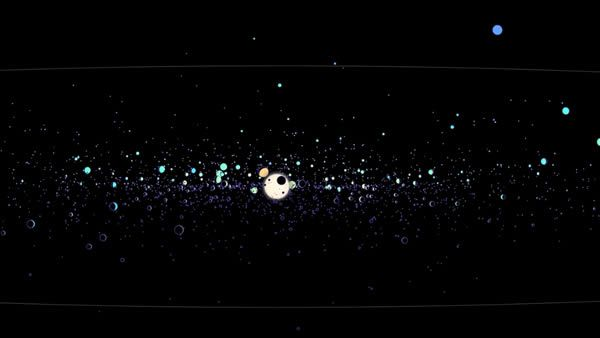
\includegraphics[width=0.8\textwidth]{images/worlds.jpg}
  \caption{Image of Worlds Visualisation}git a
\end{figure}
The layout of this animation is very similarly to the Kepler Visualisation Tool that I am extending. This means that it provides insights into how my visualisation can be improved as Worlds is a much more visually appealing system. By researching how it displays its Exoplanets I can further improve my own visualisation.
 \\\\
{\bf Scenario 1.} View planets ordered by their similarity to Earth:\\
Worlds has comprehensive functionality for comparing the different Exoplanets to one another, however it does not offer any functionality regarding comparisons to earth 
\\\\
{\bf Scenario 2.} Select ranges for attributes of each planet displayed:\\
Worlds does not offer any functionality for any filtering of Exoplanets, this means that a user can only see all planets at once which can be overwhelming and causes many of the exoplanets to be excluded from the user due to overlapping and clustering. The reason that this is done is to convey how many Exoplanets there are and how their scale differs among each Exoplanet
\\\\
{\bf Scenario 3.} Select planets to display more information:\\
Worlds is non interactive which means that users are not able to request further information about the visualisation elements that they are seeing. This ability to find out more is a key part of the interactive visualization that is needed for this project.
\\\\
{\bf Scenario 4.} View planets in the same solar system:\\
Worlds shows all Exoplanets as if they are orbiting a single star. This allows for each of them to be compared against one another easily. However this does remove the ability for a user to see which planets are together in the same solar system.
\\\\
{\bf Scenario 5.} View the Goldilocks zones of each planet:\\
Worlds does not offer this functionality.
\\\\
{\bf Scenario 6.} Select two planets to compare against one another:\\
Not applicable as worlds does not allow selections.
\\\\
{\bf Scenario 7.} Navigate the visualisation with gestures:\\
Not applicable


\subsection{The Kepler Orrery and The Kepler Orrery 2 - Non interactive}
The Kepler Orrery \cite{orrery} illustrates the exoplanet candidates in their own solar systems. The orbit radii are to scale with respect to each other and planet sizes are to scale with respect to each other, but orbits and planet sizes are different scales. The colors are in order of semi-major axis: two-planet systems (242 in all) have a yellow outer planet; 3-planet (85) green, 4-planet (25) light blue, 5-planet (8) dark blue, 6-planet (1, Kepler-11) purple. 
\begin{figure}[h!]
  \centering
      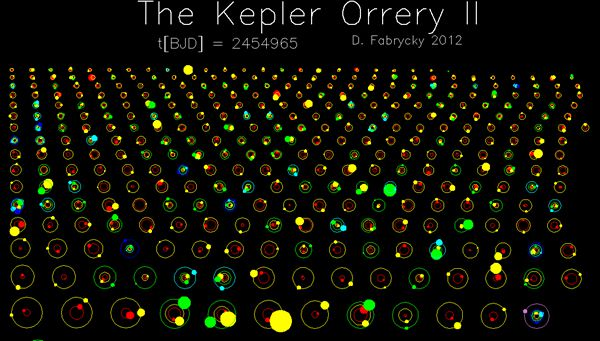
\includegraphics[width=0.8\textwidth]{images/orrery.jpg}
  \caption{Image of The Kepler Orrery Visualisation}
\end{figure}
This system exhibits small multiples, a grid of small similar graphics or charts, allowing them to be easily compared. This provides insights into how I can use small multiples to display information about groups of planets. This will be important for displaying which planets share a solar system.
\\\\
{\bf Scenario 1.} View planets ordered by their similarity to Earth:\\
Like worlds, The Kepler Orrery shows the similarities between each of the exoplanets but does not have the functionality to allow users to make a comparison to earth and our own solar system.
\\\\
{\bf Scenario 2.} Select ranges for attributes of each planet displayed:\\
As The Kepler Orrery is non interactive it is not possible to change the ranges of the Exoplanets being displayed. However due to the layout of the visualisation, which uses small multiples by grouping each solar system into its own visualisation element it removes a lot of the issue of overcrowding and overlapping.
\\\\
{\bf Scenario 3.} Select planets to display more information:\\
Not possible
\\\\
{\bf Scenario 4.} View planets in the same solar system:\\
This visualisation uses small multiples to great effect at displaying the groupings of each panel into each solar system. By displaying each planet orbiting its own star it removes the risk of confusion about what the planet is actually orbiting which could tbe the case with Worlds.
\\\\
{\bf Scenario 5.} View the Goldilocks zones of each planet:\\
Not a feature
\\\\
{\bf Scenario 6.} Select two planets to compare against one another:\\
Nope
\\\\
{\bf Scenario 7.} Navigate the visualisation with gestures: \\
Negative
\\\\

\subsection{Celestia - Interactive}
Celestia \cite{celestia} is a free real-time space simulation that lets you visually experience the universe in three dimensions. It is an open source system written in C++. 
\begin{figure}[h!]
  \centering
      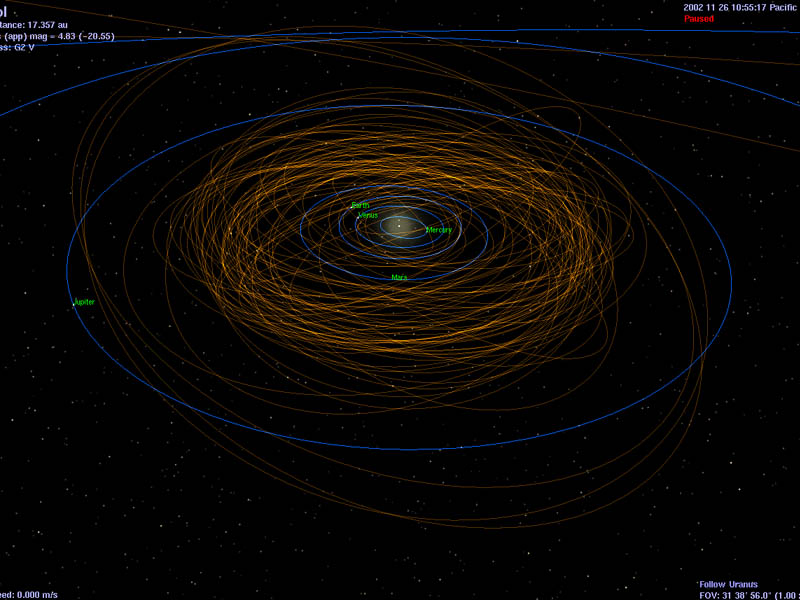
\includegraphics[width=0.5\textwidth]{images/celestia.jpg}
  \caption{Image of Celestia Visualisation}
\end{figure}
This visualisation is much larger and more encompassing system than is needed for this project, as it is a full 3D space simulation. However is does offer insights into how to effectively portray planets and their orbits (See Figure 2.3). It also provides textures that can be used in my visualisation to depict what planets actually look like to increase user immersion.
\\\\
{\bf Scenario 1.} View planets ordered by their similarity to Earth:\\
Maybe
\\\\
{\bf Scenario 2.} Select ranges for attributes of each planet displayed:\\
Maybe
\\\\
{\bf Scenario 3.} Select planets to display more information:\\
Maybe
\\\\
{\bf Scenario 4.} View planets in the same solar system:\\
Maybe
\\\\
{\bf Scenario 5.} View the Goldilocks zones of each planet:\\
Maybe
\\\\
{\bf Scenario 6.} Select two planets to compare against one another:\\
Maybe\\\\
{\bf Scenario 7.} Navigate the visualisation with gestures: \\
Maybe\\\\
\subsection{Kepler Visualisation Tool}
An existing system built with Processing is the Kepler Visualisation Tool\cite{kepler_github, kepler_article}. It is a simple visualisation focusing on displaying the candidate Exoplanets temperatures and their locations in relation to their distance from their nearest star, so that a sense of scale can be perceived. Each candidate’s estimated size, orbital speed, and orbital separation is accurately depicted, and each planet is color-coded according to its estimated effective temperature.
\begin{figure}[h!]
  \centering
      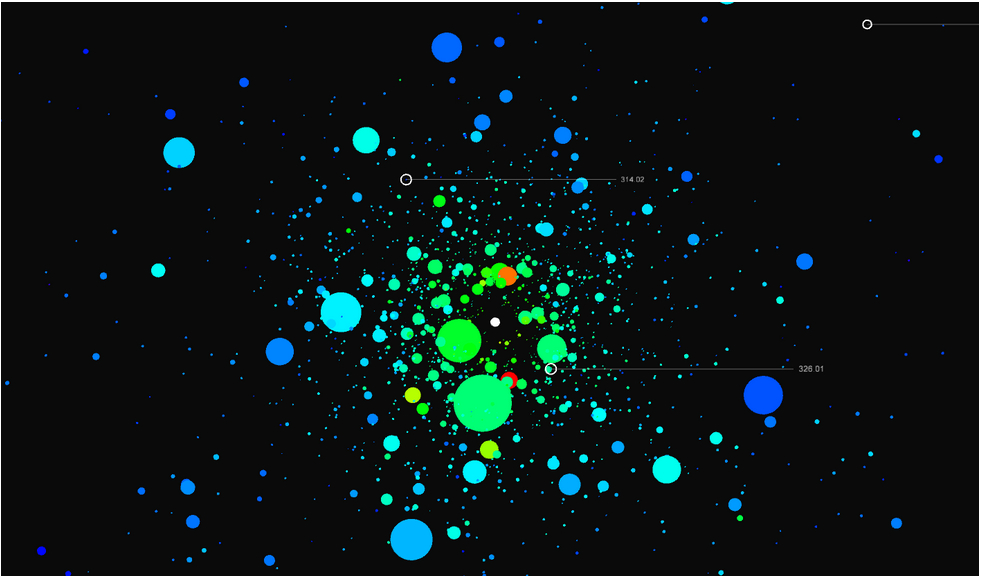
\includegraphics[width=0.8\textwidth]{images/kepler_orbital.jpg}
  \caption{Kepler Visualisation Tool Orbital View}
\end{figure}
\begin{figure}[h!]
  \centering
      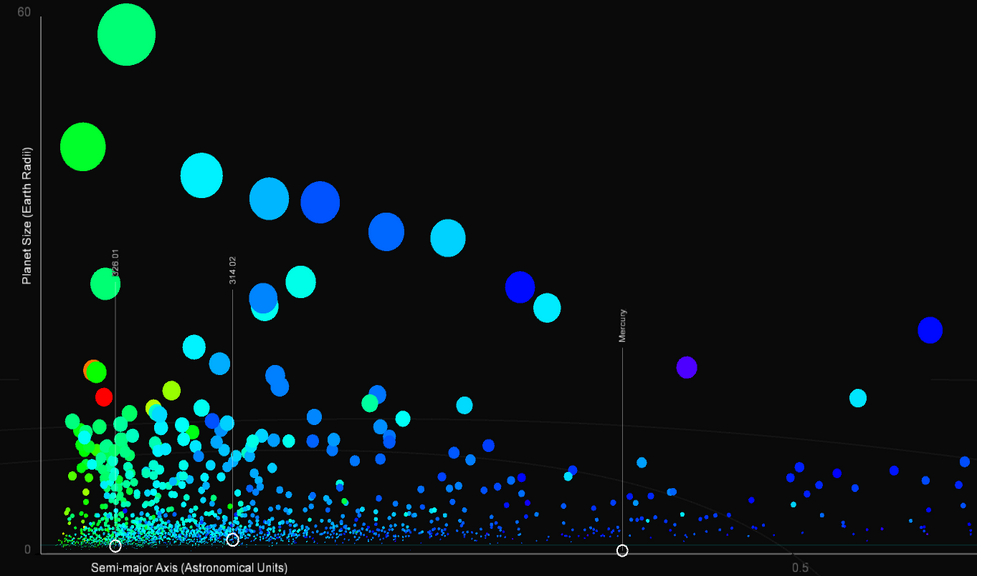
\includegraphics[width=0.8\textwidth]{images/kepler_graph.jpg}
  \caption{Kepler Visualisation Tool Graph View}
\end{figure}
The existing work in this system would serve as foundation for this project. Because much of the visual aspects, and initial data manipulation of the existing system are already complete. It means that implementing the features needed for this projects completion could be focused on more heavily and larger improvements to the existing system can be undertaken, such as better labeling and information displays and user interaction methods.
\\\\
{\bf Scenario 1.} View planets ordered by their similarity to Earth:\\
Like Worlds and the Kepler Orrery, The Kepler Visualisation Tool has functionality to display the similarity of each Exoplanet to each other. However, it also has some limmited functionality of comparing these to earth which the others lack. It does this by displaying Earthm, Mars, and Jupiter with the same colours, size, and orbit speed as the Exoplanets. This gives a user a chance to comprehend the scale and difference of some of the Exoplanets.
\\\\
{\bf Scenario 2.} Select ranges for attributes of each planet displayed:\\
The Kepler Visualisation Tool allows users to change which attributes the planets are ordered by on the vertical plane (Y axis) ie, by size or temperature, but does not allow users to select ranges of these attributes to filter the Exoplanets
\\\\
{\bf Scenario 3.} Select planets to display more information:\\
There is no selection functionality in the Kepler Visualisation Tool which means that a lot of the potential information about each Exoplanet goes undisplayed.
\\\\
{\bf Scenario 4.} View planets in the same solar system:\\
Nope
\\\\
{\bf Scenario 5.} View the Goldilocks zones of each planet:\\
Nope
\\\\
{\bf Scenario 6.} Select two planets to compare against one another:\\
Nope
\\\\
{\bf Scenario 7.} Navigate the visualisation with gestures: \\
Nope

\subsection{Summary of Existing Applications}

Matrix compared to requirements

\section{Analysis of technology options}
Many technologies were looked into,experimented with, and the positives and negatives of each weighed up before a decision was made about which would be the choice for the visualisation. It came down to 3 potential technologies that would be suitable for the project, the next 3 subsections outline these in detail.

\subsection{D3 (Data Driven Documents)}
D3 is a JavaScript library that allows the displaying of data in dynamic graphics. Embedded
within an HTML web page, the JavaScript D3.js library uses pre-built JavaScript functions to
select elements, create Scalable Vector Graphic (SVG)[17] objects, style them, and add transitions,
dynamic effects and tooltips. Large datasets can be easily bound to SVG objects using
simple D3 functions to generate rich charts and diagrams. D3 was created because of the
need for a balance of expressiveness, efficiency, and accessibility that previous visualization
toolkits did not allow [4].

D3 allows the binding of input data to arbitrary input elements. This means that the exoplanet
dataset can easily be bound to SVG elements for creating visualizations. D3 adopts
the W3C Selectors API to identify document elements queried. This results in a rich but
concise selection method of elements in a visualisation.

D3 allows debugging thanks to Google chrome and other modern browsers development
tools. A downside to D3 is that it does not allow 3D diagrams, although it does allow
pseudo 3D by using the painter’s algorithm and 3D textures.

\subsection{Prefuse}
Prefuse is a set of software tools for creating rich interactive data visualizations [13]. The
Prefuse toolkit provides a visualization framework for Java. It supports a set of features
for visualizing and interacting with data. It provides optimized data structures for tables,
graphs, and trees. It can be used to build standalone applications, visual components embedded
in larger applications, and web applets. Prefuse to greatly simplifies the process
of representing and efficiently handling data, mapping data to visual representations (e.g.,
through spatial position, size, shape, color, etc), and interacting with the data.
To use Prefuse a basic familiarity with the Java is required, including setting up and building
Java projects. A knowledge of Swing or another similar user interface toolkit is also
useful for understanding some of the concepts behind Prefuse and for integrating Prefuse
visualizations into larger applications. Experience with database systems is also helpful. 
However the complexity of Prefuse means that the learning curve will be out of scope for
this project.

\subsection{Processing}
Processing is an open source programming language and development environment that was initially created to serve as a software
sketchbook and to teach the fundamentals of computer programming with a visual context.
Using processing would mean that the visualization could be built with Java while still using
a successful visualisation framework. The most complete existing visualization using
the same exoplanet dataset (Kepler Visualization Tool) is built using Processing.
Using this solution would involve learning the Processing language, however Processing
is a library built in Java so the syntax is the same. This means the learning curve should be shallow.
Using processing means that 3D elements could be included, this wouldnt be
possible with D3.

\subsection{Decision of technology}
The final decsion of techology was to use Processing, this is because it had many positive aspects that the others did not and minimal nigatives as the below table illistrates.
\clearpage
\begin{figure}[h!]
  \centering
      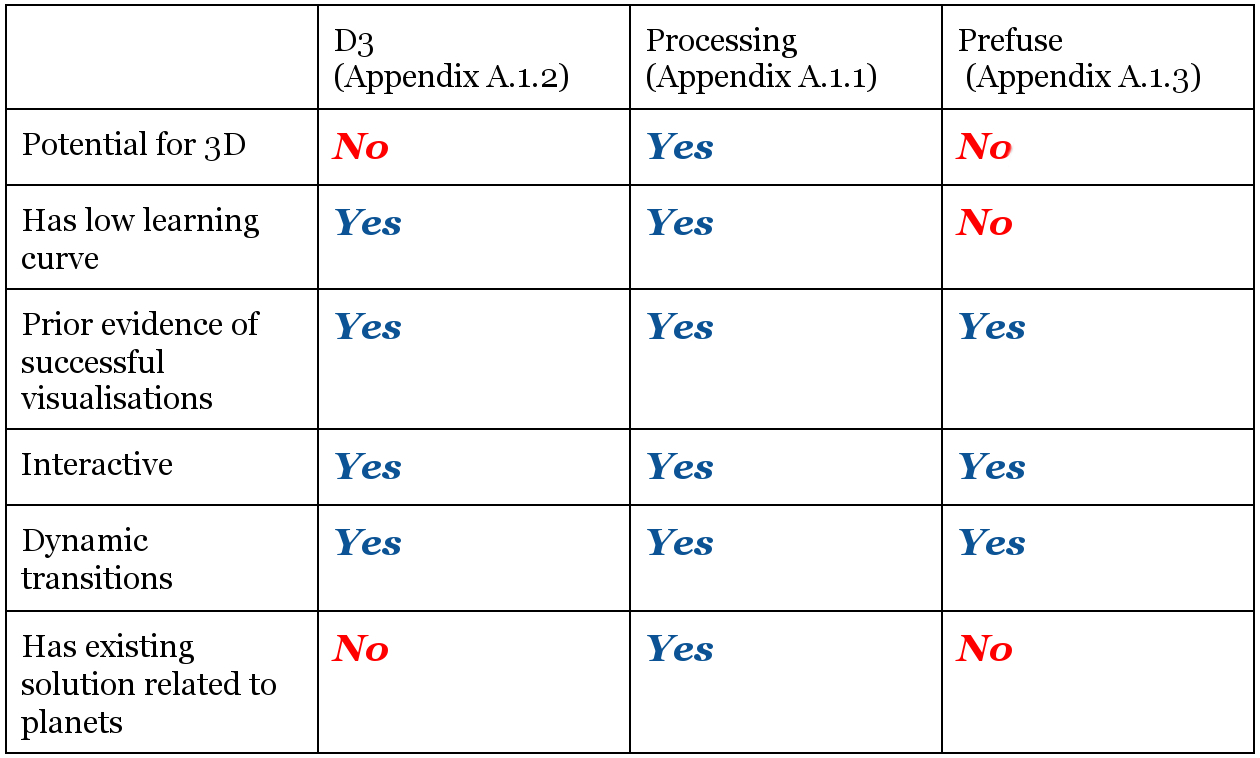
\includegraphics[width=0.8\textwidth]{images/table_technologies.jpg}
  \caption{Table of technology choices}
\end{figure}

As this project was created using Processing, it allowed me to extend the previous visualisation using the same data set, The Kepler Visualisation Tool \cite{kepler_github, kepler_article}. As the time was short for this project builing upon a previous solution increased the amount of progress that could be made in the time afforded.
\\\\
Taking this approach meant that the languages being used would be Java using processing libraries. 

As this is such a large project involving many different iterations, version control was important for maintaining records and backups of important changes which was stored on remote servers to ensure against file loss in system failures.